\section{Arquitectura del sistema}

\subsection{Contexto del sistema}
SREI lo usan cinco tipos de personas. Cuatro pertenecen a la UTEQ: 
el docente que propone los eventos, el coordinador de carrera que los 
aprueba o rechaza, el decano que los supervisa y los estudiantes que consultan los eventos y confirman su asistencia.
El quinto es el usuario externo, una persona de fuera de la universidad que se registra y confirma su asistencia. 
SREI se relaciona con un solo sistema externo, un servicio de IA generativa que crea la imagen de un evento 
a partir de la descripción que escribe el docente (Figura~\ref{fig:c4-contexto}).

\begin{figure}[H]
  \centering
  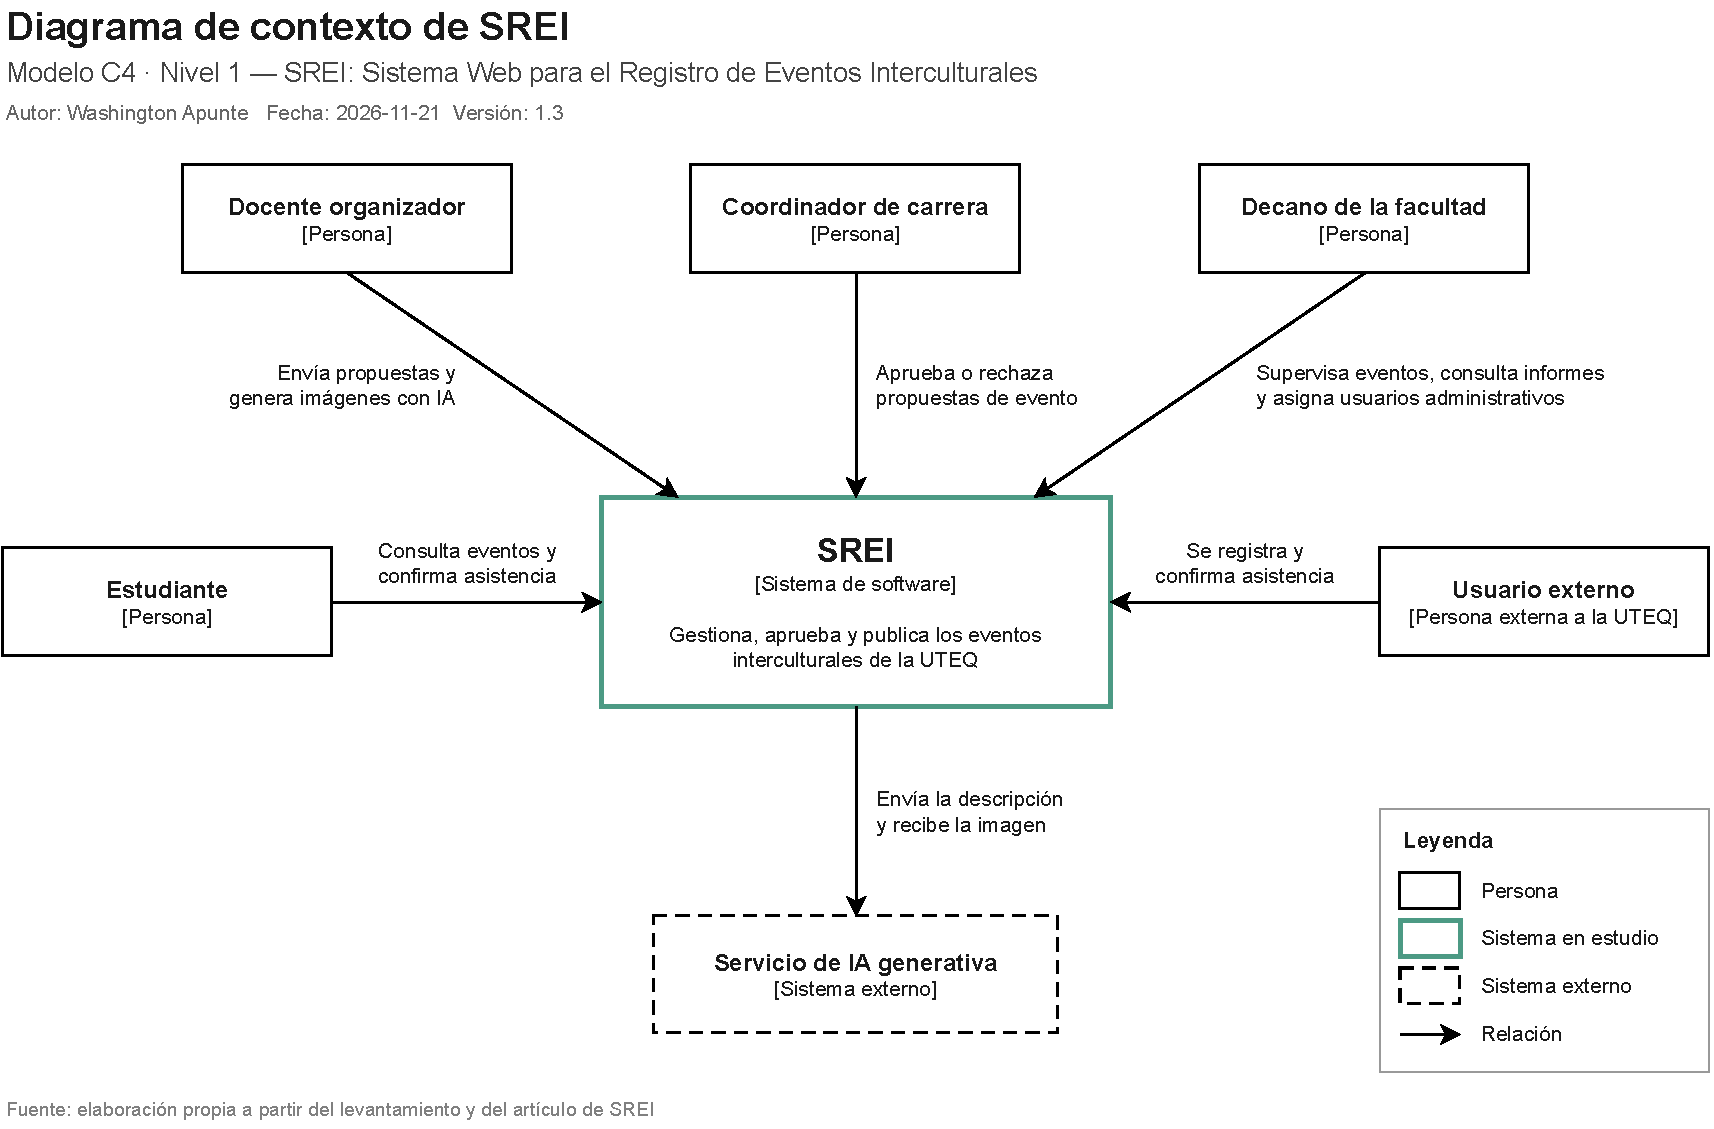
\includegraphics[width=\textwidth]{diagramas/c4-contexto.pdf}
  \caption{Diagrama de contexto (C4, nivel 1). Fuente: elaboración propia.}
  \label{fig:c4-contexto}
\end{figure}

\subsection{Contenedores}
La Figura~\ref{fig:c4-contenedores} muestra lo que hay dentro de SREI. 
Los usuarios entran por una aplicación web hecha en Angular 17, 
que se comunica con tres servicios Spring Boot: servicio-eventos en el puerto 8080, 
servicio-consulta en el puerto 8081 y servicio-usuarios. 
En el diseño, cada servicio guarda sus datos en su propia base PostgreSQL. 
Por ahora solo funcionan servicio-eventos y servicio-consulta, con el enlace INT-01, 
por el que servicio-consulta le pide los datos de un evento a servicio-eventos. 
La aplicación web, servicio-usuarios, las tres bases de datos y los demás enlaces todavía están previstos,
por eso se dibujan con línea punteada. 
El servicio de IA queda fuera de la frontera del sistema y se conectará desde servicio-eventos.

\begin{figure}[p]
  \centering
  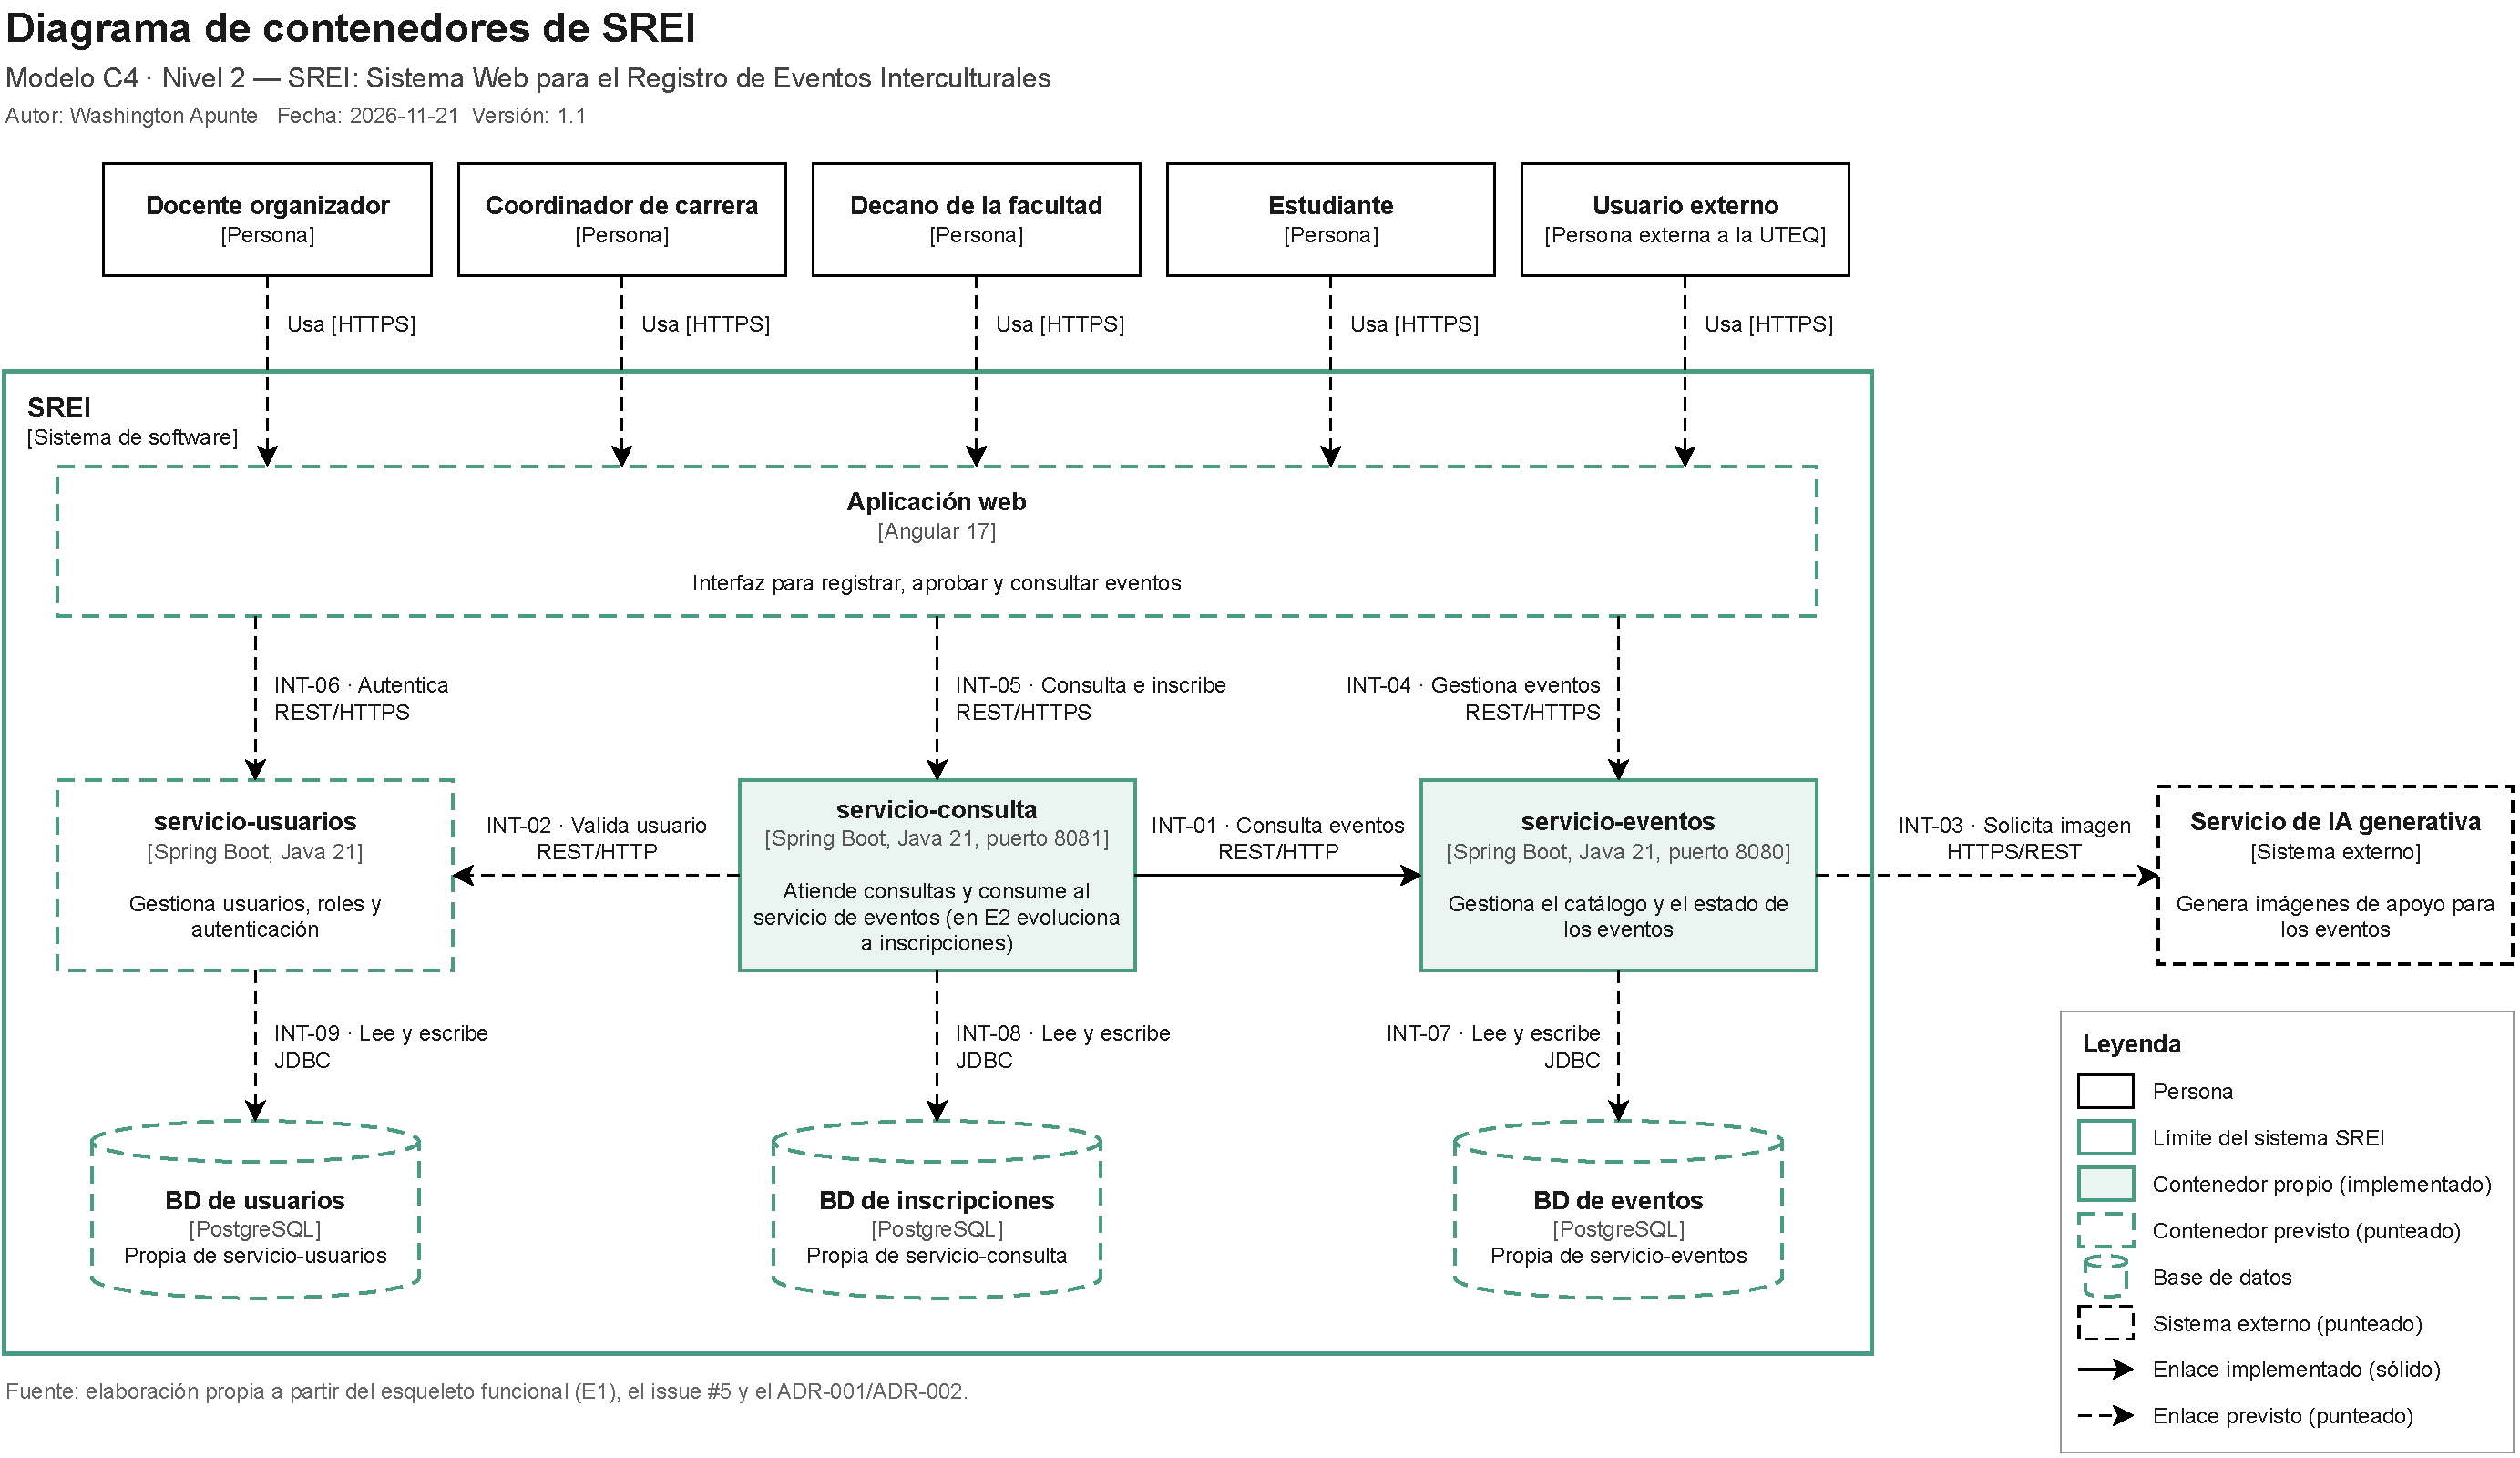
\includegraphics[width=0.9\textheight, height=0.85\textwidth, keepaspectratio, angle=90]{diagramas/c4-contenedores.pdf}
  \caption{Diagrama de contenedores (C4, nivel 2). Fuente: elaboración propia.}
  \label{fig:c4-contenedores}
\end{figure}

\subsection{Por qué un sistema distribuido y no un monolito}
Hoy SREI es un monolito: un solo backend y una sola base de datos hacen todo el trabajo. 
El problema es que una parte lenta frena a las demás. Puede pasar, por ejemplo, con la generación de imágenes, 
que depende de un servicio de IA que no controlamos. Mientras la IA no responde, 
cada petición sigue ocupando un hilo del mismo servidor que atiende el inicio de sesión y las inscripciones. 
Cuando esas esperas se acumulan, el servidor ya no tiene hilos para atender a nadie más y todo SREI se vuelve lento. 
Además, el PFC exige un sistema distribuido, y un monolito no lo es.

Con tres servicios, cada uno corre por separado y es dueño de su base de datos. 
La llamada a la IA saldrá solo de servicio-eventos (INT-03, previsto), así que si la IA se pone lenta, 
el problema se queda en ese servicio. El inicio de sesión, que maneja servicio-usuarios, sigue funcionando, 
y servicio-consulta solo se ve afectado cuando necesita datos de eventos. Separar los datos también ayuda. 
Como ningún servicio lee la base de otro, un cambio en las tablas de eventos no obliga a tocar las de inscripciones o usuarios.

Esta decisión tiene costos que aceptamos. Hay más piezas que levantar y configurar, 
cada una con su puerto y su base. Ya no se pueden unir datos de distintos servicios con un JOIN, 
así que hay que pedirlos por la API. Y como los servicios se llaman de forma síncrona, si servicio-eventos se cae, 
servicio-consulta no puede completar la consulta y el usuario ve un error.

Las opciones consideradas y la decisión completa están en el ADR-001.